%!TEX root = ../../thesis.tex

The analysis is jet-binned since the background composition strongly depends upon jet 
multiplicity (see \Figure\ref{fig:sel:njets}). There are 0-jet and 1-jet bins, and a 
\twojet bin split into ggF and VBF signal regions (see 
\Figure~\ref{fig:sig:jetbinning}). Uncertainties should be evaluated separately for each 
bin, and correlations accounted for when the bins are combined. Perturbative 
uncertainties require particular consideration, due to subtleties described below.

\begin{figure}
	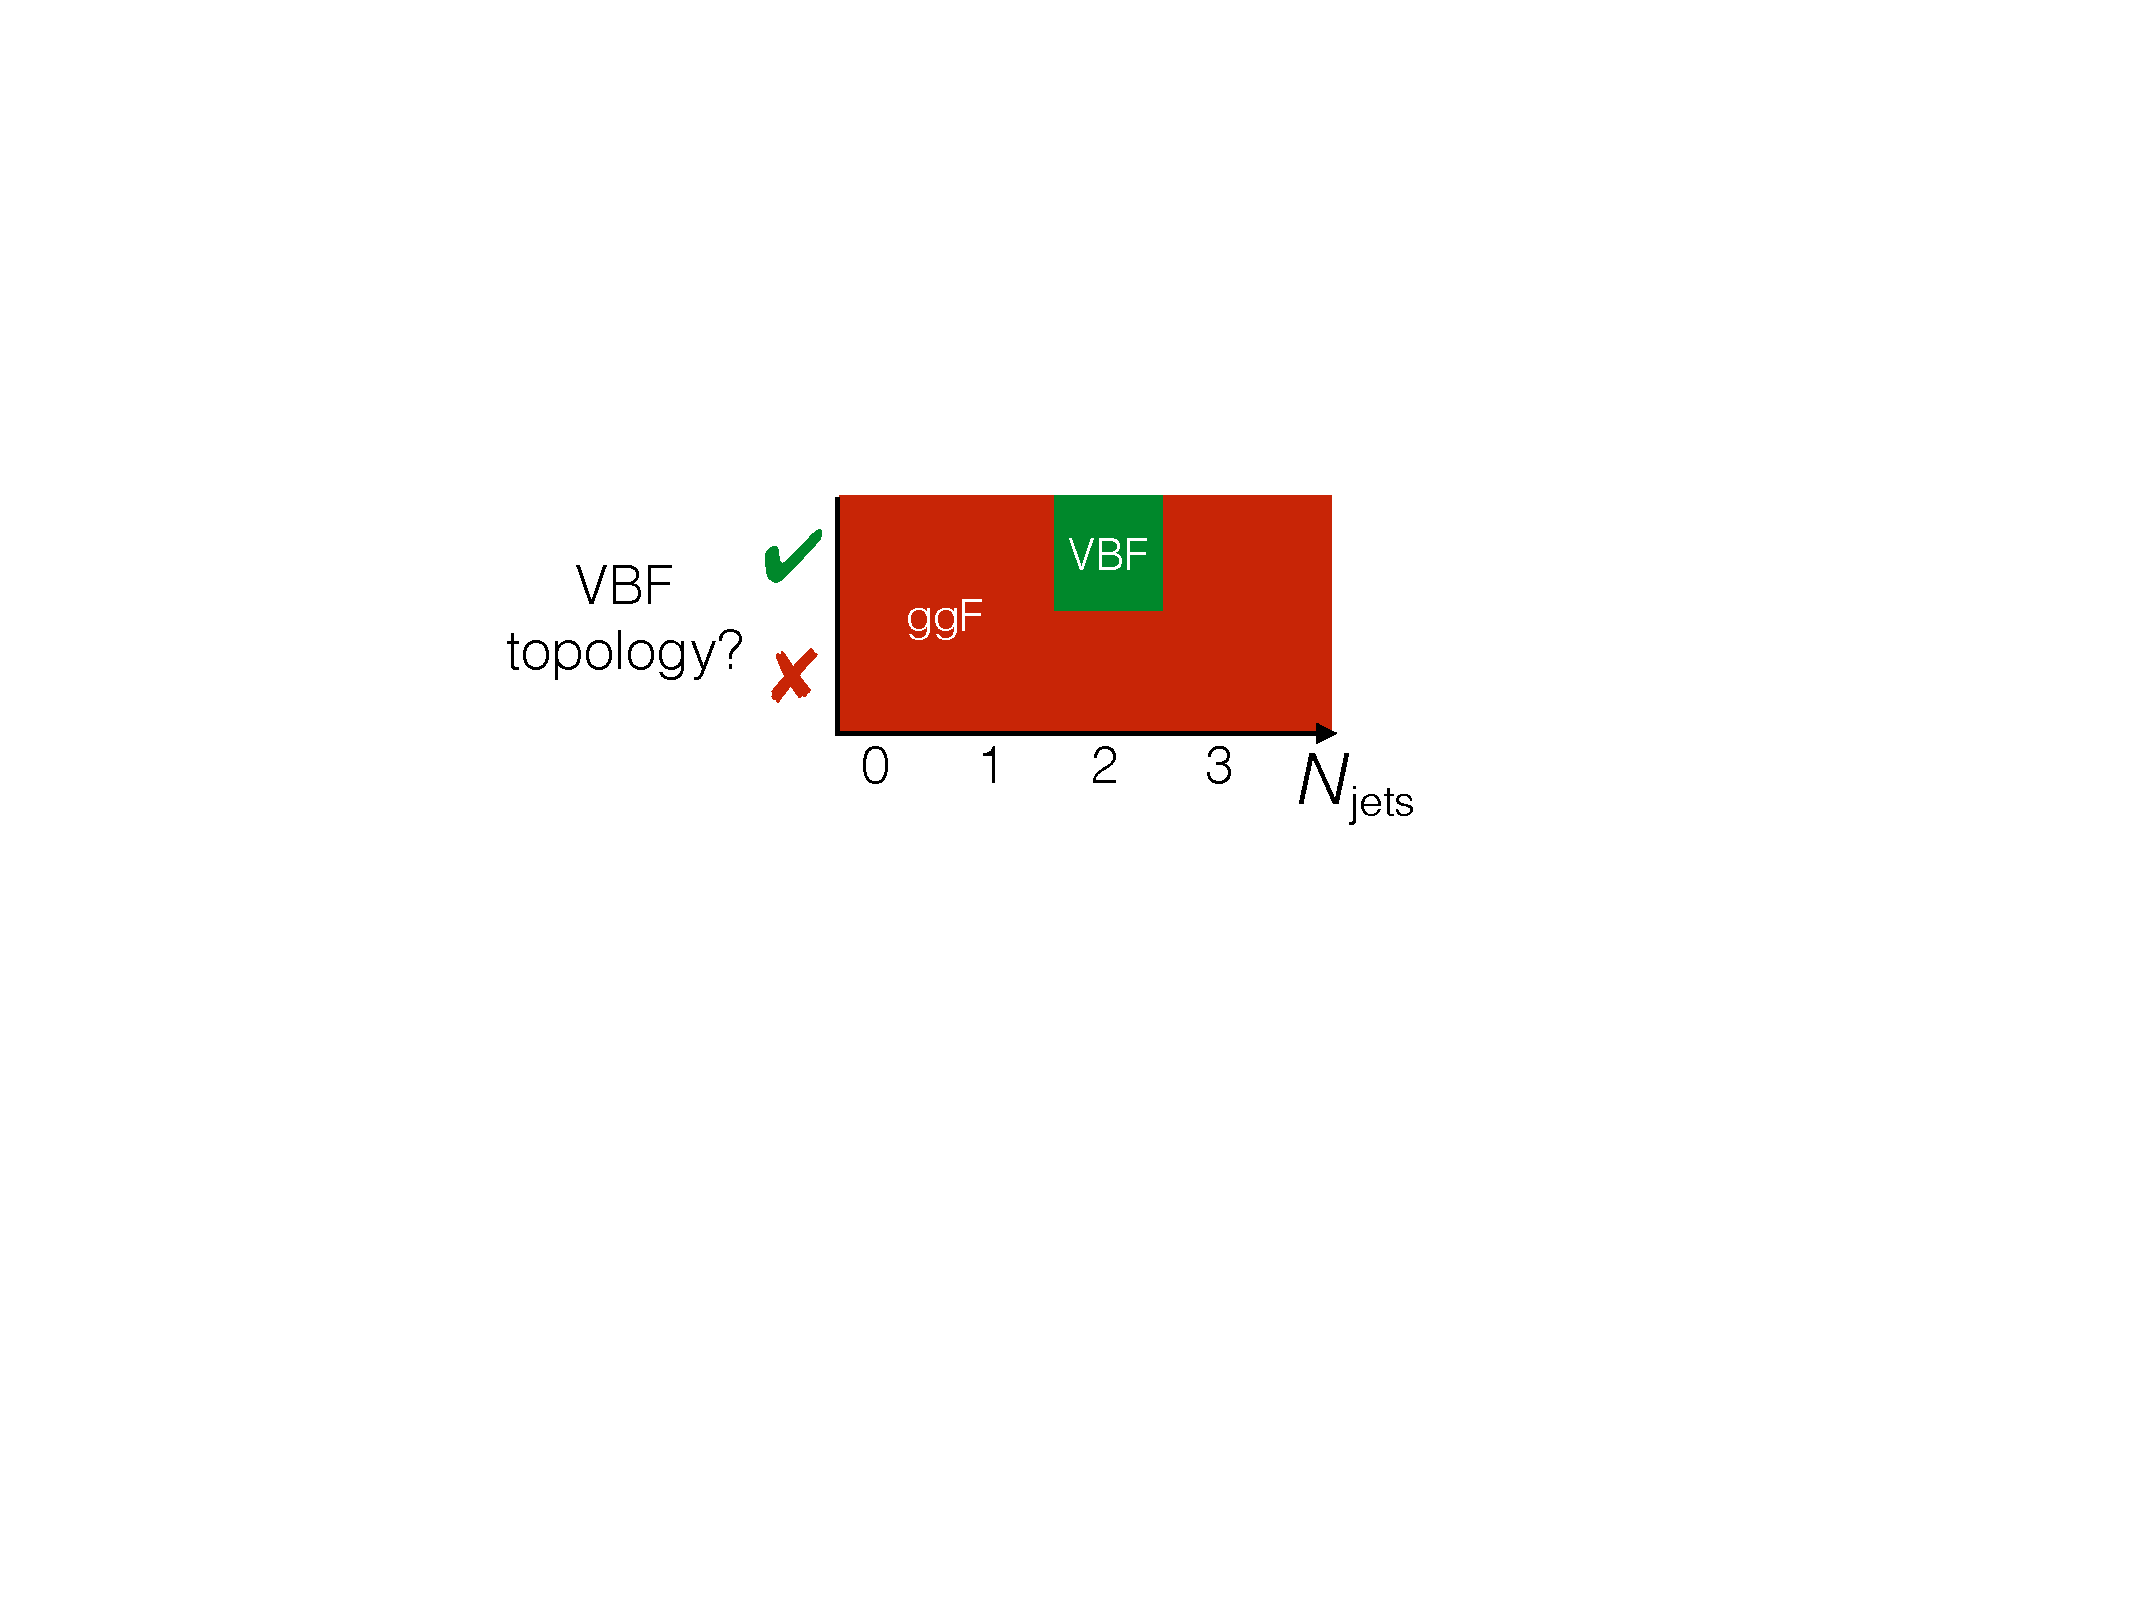
\includegraphics[width=\mediumfigwidth,clip=true,trim=8.5cm 13.1cm 12.1cm 8.4cm]{custom_images/signal_jetbin}
	\caption{Schematic diagram of the ggF and VBF signal regions. Note that the 
	exclusivity of the VBF signal region is defined by a central jet veto, and thus 
	for $\njets \geq 3$ the jet definition includes the restriction that $\eta$ is 
	between $\eta_{j_1}$ and $\eta_{j_2}$.}
	\label{fig:sig:jetbinning}
\end{figure}



\subsection{Perturbative uncertainties in jet-binned cross sections}
\label{sec:ggF:naive}

Consider splitting a cross section into two parts: an exclusive $\sigma_0$ and an 
inclusive $\sigma_{\geq1}$
\begin{equation}
	\sigma_{\total} = \sigma_0 \parenths{\ptcut} + \sigma_{\geq1} \parenths{\ptcut}
\end{equation}
where \ptcut is the jet \pt threshold \cite{YR2}. In $\sigma_{\geq1}$, the requirement of 
a jet with $\pt > \ptcut$ introduces Sudakov double logarithmic contributions 
$\alpha_{\text{S}}^{k+m} L^{2m}$, where $L \sim \ln\parenths{\ptcut/Q}$ ($Q = \mH$ for 
ggF). These are analogous to the logarithms introduced by soft gluon emission, 
described in \Section~\ref{sec:qcd:resum}. 

The schematic structures of the two inclusive cross sections are
\begin{equation}
	\sigma_{\total} &\sim \alpha_{\text{S}}^k \{1 &+& \alphaS &+& \alpha_{\text{S}}^2 &+& \ofOrder{\alpha_{\text{S}}^3}\} \\
\sigma_{\geq1}  &\sim \alpha_{\text{S}}^k \{&\phantom{{}=+}&\alphaS (L^2 + L + 1) &+& \alpha_{\text{S}}^2 (L^4 + L^3 + L^2 + L + 1) &+& \ofOrder{\alpha_{\text{S}}^3 L^6}\}
\end{equation}
and the exclusive cross section is $\sigma_0 = \sigma_{\total} - \sigma_{\geq1}$.
Corrections to $\sigma_{\total}$ are large (see \Section~\ref{sec:ggf_inc}) and, when 
$\ptcut \ll \mH$, the logarithms can overcome the \alphaS suppression and provide 
significant corrections to $\sigma_{\geq1}$ too. Cancellations then occur between the two 
series and the scale dependence of $\sigma_0$ is reduced. This effect is rather extreme 
near \unit{$\ptcut = 25$}{\GeV} (see \Figure~\ref{fig:signal:ggf_sigma0_CI}), as used in 
the \HWW analysis . Clearly na\"{i}ve scale variations are unsuitable for evaluating 
perturbative uncertainties.

When discussing uncertainties in jet-binned cross sections, it is convenient to consider 
a general parametrisation of the covariance matrix. In the \braces{\sigma_0, 
\sigma_{\geq1}} basis, the covariance matrix is decomposed into two uncertainty sources
\begin{equation}
	C &= C^{\text{yield}} + C^{\text{migration}} \\
	&= \twomatrix{\parenths{\Delta^{\text{y}}_0}^2 & \Delta^{\text{y}}_0 \Delta^{\text{y}}_{\geq1}}{\Delta^{\text{y}}_0 \Delta^{\text{y}}_{\geq1} & \parenths{\Delta^{\text{y}}_{\geq1}}^2} + \parenths{\Delta_{0\rightarrow}^{\text{mig}}}^2\twomatrix{1 & -1}{-1 & 1} \,.
\end{equation}
The yield component is fully correlated, though can affect the two bins with different 
magnitudes. The migration component is fully anti-correlated, and affects both bins 
equally so that normalisation is conserved. In the limit setting procedure, these sources 
are treated as nuisance parameters with uncertainty amplitudes
\begin{equation}
	\begin{array}{l@{}l@{}l}
		\begin{array}{r}
			\kappa^{\text{yield}}              : \Big( \\
			\kappa^{\text{mig}}_{0\rightarrow} : \Big(
		\end{array}
		&
		\begin{array}{@{}rrr@{}}
			\Delta^{\text{y}}_0, & \Delta^{\text{y}}_{\geq1} \\
			\Delta^{\text{mig}}_{0\rightarrow}, & -\Delta^{\text{mig}}_{0\rightarrow}
		\end{array}
		&
		\begin{array}{l}
			\Big) \\ \Big) \,.
		\end{array}
	\end{array}
	\label{eq:ggF:2bin_np}
\end{equation}

Note that so far we have remained fairly general and $\Delta^{\text{y}}_0$, 
$\Delta^{\text{y}}_{\geq1}$ and $\Delta^{\text{mig}}_{0\rightarrow}$ remain undetermined. 
We shall see that different methods of evaluating perturbative uncertainties shall 
effectively determine these uncertainty amplitudes. For example, the na\"{i}ve method 
described above is equivalent to choosing
\begin{equation}
	\text{Na\"{i}ve:} 
	\quad\quad \Delta^{\text{y}}_0 &= \Delta\sigma_{0},& 
	\quad\quad \Delta^{\text{y}}_{\geq1} &= \Delta\sigma_{\geq1},&
	\quad\quad \Delta^{\text{mig}}_{0\rightarrow} &= 0
\end{equation}
where uncertainties are evaluated at fixed order via scale variations.

In the \HWW analysis, there is also a 1-jet exclusive bin. The second jet veto introduces 
an additional source of migrations, now between the 1-jet and \twojet bins. 
Therefore, in the \braces{\sigma_0, \sigma_1, \sigma_{\geq2}} basis, the covariance 
matrix has three components
\begin{equation}
	C &= 
	\threematrix{
		\parenths{\Delta^{\text{y}}_0}^2 & 
		\Delta^{\text{y}}_0 \Delta^{\text{y}}_1 & 
		\Delta^{\text{y}}_0 \Delta^{\text{y}}_{\geq2}
	}{
		\Delta^{\text{y}}_0 \Delta^{\text{y}}_1 & 
		\parenths{\Delta^{\text{y}}_1}^2 & 
		\Delta^{\text{y}}_1 \Delta^{\text{y}}_{\geq2}
	}{
		\Delta^{\text{y}}_0 \Delta^{\text{y}}_{\geq2} & 
		\Delta^{\text{y}}_1 \Delta^{\text{y}}_{\geq2} & 
		\parenths{\Delta^{\text{y}}_{\geq2}}^2
	}
	\nonumber \\
	&+ \parenths{\Delta^{\text{mig}}_{0\rightarrow}}^2
	\threematrix{
		1 & -\parenths{1-\rho} & -\rho
	}{
		-\parenths{1-\rho} & \parenths{1-\rho}^2 & \rho\parenths{1-\rho}
	}{
		-\rho & \rho\parenths{1-\rho} & \rho^2
	}
	+ \parenths{\Delta^{\text{mig}}_{1\rightarrow}}^2
	\threematrix{
		0 & 0 & 0
	}{
		0 & 1 & -1
	}{
		0 & -1 & 1
	}
\end{equation}
where $\rho$ is the fraction of migrations from the 0-jet bin that enter the 
\twojet bin. In the 3-bin case, there are three nuisance parameters with 
uncertainty amplitudes
\begin{equation}
	\begin{array}{l@{}l@{}l}
		\begin{array}{r}
			\kappa^{\text{yield}}              : \Big( \\
			\kappa^{\text{mig}}_{0\rightarrow} : \Big( \\
			\kappa^{\text{mig}}_{1\rightarrow} : \Big(
		\end{array}
		&
		\begin{array}{@{}rrr@{}}
			\Delta^{\text{y}}_0, & \Delta^{\text{y}}_1, & \Delta^{\text{y}}_{\geq2} \\
			\Delta^{\text{mig}}_{0\rightarrow}, & -\parenths{1-\rho} \Delta^{\text{mig}}_{0\rightarrow}, & -\rho \Delta^{\text{mig}}_{0\rightarrow} \\
			0, & \Delta^{\text{mig}}_{1\rightarrow}, & -\Delta^{\text{mig}}_{1\rightarrow}
		\end{array}
		&
		\begin{array}{l}
			\Big) \\ \Big) \\ \Big) \,.
		\end{array}
	\end{array}
	\label{eq:ggF:3bin_np}
\end{equation}
So it is $\Delta^{\text{y}}_0$, $\Delta^{\text{y}}_1$, $\Delta^{\text{y}}_{\geq2}$, 
$\Delta^{\text{mig}}_{0\rightarrow}$, $\Delta^{\text{mig}}_{1\rightarrow}$ and $\rho$ 
that must be determined. Two different methods for evaluating these shall now be examined.



\subsection{Combined inclusive method}
\label{sec:ggF:ci}

The \textit{combined inclusive} (CI) method\footnote{
	The CI method is also called the Stewart-Tackmann method, after its original 
	proponents.
} \cite{Stewart-Tackmann:2012} uses scale variations of $\sigma_{\geq1}$ and 
$\sigma_{\geq2}$ to probe the size of the higher order logarithmic corrections, and 
identifies that they are related to the bin migration uncertainties. It therefore chooses
\begin{equation}
	\text{CI:}
	\quad\quad \Delta^{\text{y}}_0 &= \Delta\sigma_{\total},&
	\quad\quad \Delta^{\text{y}}_1 &= 0,&
	\quad\quad \Delta^{\text{y}}_{\geq2} &= 0, \nonumber \\
	\quad\quad \Delta^{\text{mig}}_{0\rightarrow} &= \Delta\sigma_{\geq1},&
	\quad\quad \Delta^{\text{mig}}_{1\rightarrow} &= \Delta\sigma_{\geq2},&
	\quad\quad \rho &= 0
\end{equation}
where uncertainties are evaluated at fixed order via scale variations. Actually, 
$\Delta\sigma_{\total}$ is taken from the calculations described in 
\Section~\ref{sec:ggf_inc}, rather than fixed order.

This is equivalent to assuming inclusive cross sections have uncorrelated uncertainties
\begin{equation}
	\text{CI:} \quad\quad
	\sigma_N = \sigma_{\geq N} - \sigma_{\geq N+1}
	\quad\quad\Rightarrow\quad\quad
	\Delta\sigma_N^2 = \Delta\sigma_{\geq N}^2 + \Delta\sigma_{\geq N+1}^2 \,.
\end{equation}
Although this assumption is not believed to be exact, the CI method offers a practical 
solution to the cancellations observed with the na\"{i}ve method (see 
\Figure~\ref{fig:signal:ggf_sigma0_CI}). Uncertainties in $\sigma_{N}$ must be at least 
as large as those in $\sigma_{\geq N}$, and the large-\ptcut limit is correct. 

It should be noted that each inclusive cross section must be evaluated at the same order 
in \alphaS (\eg $\sigma_{\total}^{\text{NNLO}}$, $\sigma_{\geq1}^{\text{NLO}}$ and 
$\sigma_{\geq2}^{\text{LO}}$). In the case of ggF contamination to the VBF 
signal region, the uncertainties are evaluated in a significantly different region of 
phase space, and so are treated as uncorrelated.

\begin{figure}
	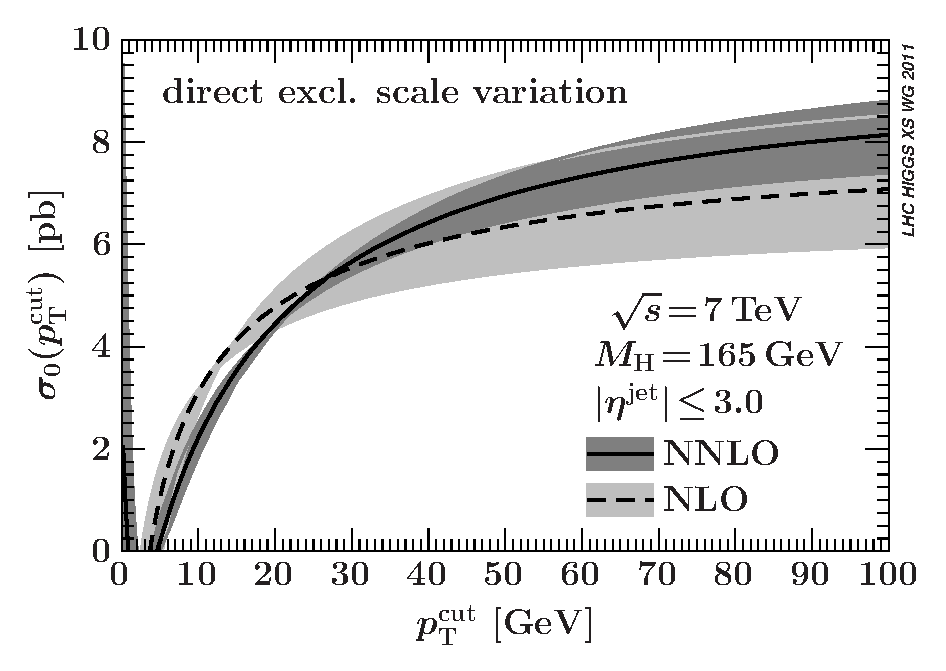
\includegraphics[width=0.495\textwidth]{tex/signal/sigma0_naive}
	\hfill
	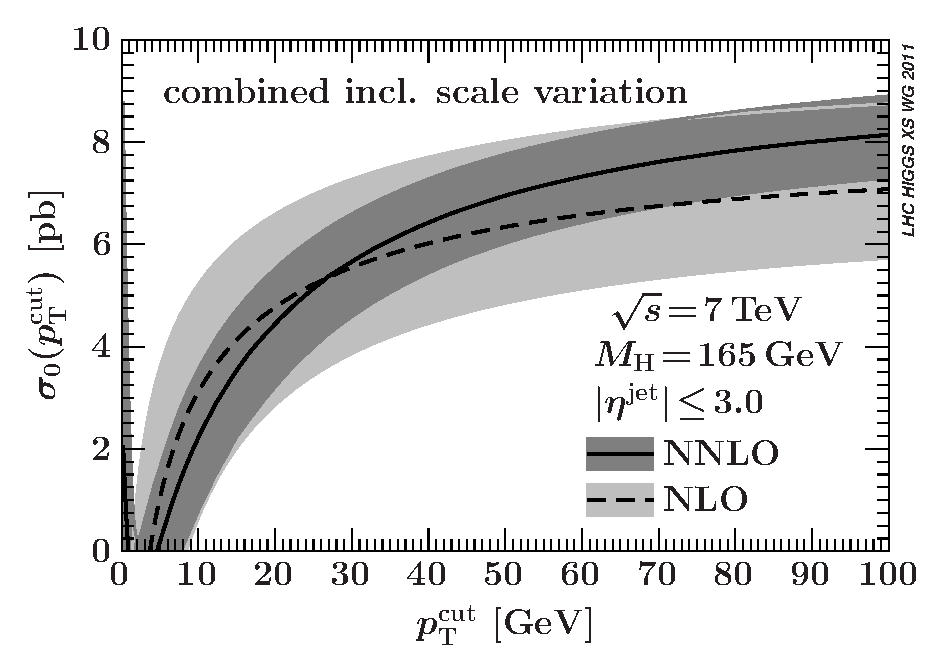
\includegraphics[width=0.495\textwidth]{tex/signal/sigma0_CI}
	\caption{The 0-jet exclusive ggF cross section versus the jet \pt threshold 
	\cite{YR2}. The band shows the perturbative uncertainties evaluated using the 
	na\"{i}ve method (left) and the combined inclusive method (right).}
	\label{fig:signal:ggf_sigma0_CI}
\end{figure}


\subsection{Jet veto efficiency method}
\label{sec:ggF:jve}

The \textit{jet veto efficiency} (JVE) method \cite{JVE:NLL} takes quite a different 
approach. It considers each exclusive cross section as a product of the total cross 
section and jet veto efficiencies
\begin{equation}
	\sigma_0 &= \sigma_{\total} \epsilon_0 \\
	\sigma_1 &= \sigma_{\total} \parenths{1-\epsilon_0} \epsilon_1 \\
	\sigma_{\geq2} &= \sigma_{\total} \parenths{1-\epsilon_0} \parenths{1-\epsilon_1}
\end{equation}
where $\epsilon_0 = \epsilon_0\parenths{\ptcut}$ and 
$\epsilon_1 = \epsilon_1\parenths{p_{\text{T}}^{\text{sel}}, \ptcut}$ are the first and 
second jet veto efficiencies. It then assumes that uncertainties in $\sigma_{\total}$ and 
$\epsilon_N$ are uncorrelated, and therefore exclusive cross sections must have an 
uncertainty at least as large as $\Delta\sigma_{\total}$. This is equivalent to
\begin{equation}
	\text{JVE:}
	\quad\quad \Delta^{\text{y}}_0 &= \Delta\sigma_{\total} \, \frac{\sigma_{0}}{\sigma_{\total}} \,,&
	\quad\quad \Delta^{\text{y}}_1 &= \Delta\sigma_{\total} \, \frac{\sigma_{1}}{\sigma_{\total}} \,,&
	\quad\quad \Delta^{\text{y}}_{\geq2} &= \Delta\sigma_{\total} \, \frac{\sigma_{\geq2}}{\sigma_{\total}} \,, \nonumber \\
	\quad\quad \Delta^{\text{mig}}_{0\rightarrow} &= \Delta\epsilon_0 \, \sigma_{\total} \,,&
	\quad\quad \Delta^{\text{mig}}_{1\rightarrow} &= \Delta\epsilon_1 \, \sigma_{\geq1} \,,&
	\quad\quad \rho &= 1-\epsilon_1 \,.
\end{equation}
Again, $\Delta\sigma_{\total}$ is taken from \Section~\ref{sec:ggf_inc}. However, 
$\epsilon_N$ contains similar cancellations to those discussed in 
\Section~\ref{sec:ggF:naive}, and so $\Delta\epsilon_N$ must be treated with care.

There is an ambiguity in the definition of $\epsilon_N$ that is not present in fixed 
order calculations. For example, at NNLO, three alternative definitions of 
$\epsilon_N$ may be identified
\begin{equation}
	\epsilon_N^{\parenths{\text{a}}} &= 1 - \frac{\sigma_{\geq N+1}^{\text{NLO}}}{\sigma_{\geq N}^{\text{NNLO}}} \\
	\epsilon_N^{\parenths{\text{b}}} &= 1 - \frac{\sigma_{\geq N+1}^{\text{NLO}}}{\sigma_{\geq N}^{\text{NLO}}} \\
	\epsilon_N^{\parenths{\text{c}}} &= 1 - \frac{\sigma_{\geq N+1}^{\text{NLO}}}{\sigma_{\geq N}^{\text{LO}}} + \parenths{\frac{\sigma_{\geq N}^{\text{NLO}}}{\sigma_{\geq N}^{\text{LO}}} - 1} \frac{\sigma_{\geq N+1}^{\text{LO}}}{\sigma_{\geq N}^{\text{LO}}} \,.
\end{equation}
Schemes (a), (b) and (c) differ by N$^3$LO terms, and therefore can probe higher 
order corrections. In processes where convergence is well behaved, \eg 
\HepProcess{\Pquark\APquark \HepTo \PZ}, these schemes converge. Therefore, 
$\epsilon_N^{\parenths{\text{a}}}$ is taken as the central value and $\Delta\epsilon_N$ 
is taken as the difference between the schemes or the scale variations in 
$\epsilon_N^{\parenths{\text{a}}}$, whichever is larger.

\todo[inline]{allows you to improve accuracy of components independently. insert plot showing resummation improvement}


\subsection{Results}
